\documentclass[]{article}
\usepackage{lmodern}
\usepackage{amssymb,amsmath}
\usepackage{ifxetex,ifluatex}
\usepackage{fixltx2e} % provides \textsubscript
\ifnum 0\ifxetex 1\fi\ifluatex 1\fi=0 % if pdftex
  \usepackage[T1]{fontenc}
  \usepackage[utf8]{inputenc}
\else % if luatex or xelatex
  \ifxetex
    \usepackage{mathspec}
  \else
    \usepackage{fontspec}
  \fi
  \defaultfontfeatures{Ligatures=TeX,Scale=MatchLowercase}
\fi
% use upquote if available, for straight quotes in verbatim environments
\IfFileExists{upquote.sty}{\usepackage{upquote}}{}
% use microtype if available
\IfFileExists{microtype.sty}{%
\usepackage{microtype}
\UseMicrotypeSet[protrusion]{basicmath} % disable protrusion for tt fonts
}{}
\usepackage[margin=1in]{geometry}
\usepackage{hyperref}
\hypersetup{unicode=true,
            pdftitle={Project Technical Discussion: Prediction of lower-body strains in Soccer},
            pdfauthor={Tamas Koncz},
            pdfborder={0 0 0},
            breaklinks=true}
\urlstyle{same}  % don't use monospace font for urls
\usepackage{longtable,booktabs}
\usepackage{graphicx,grffile}
\makeatletter
\def\maxwidth{\ifdim\Gin@nat@width>\linewidth\linewidth\else\Gin@nat@width\fi}
\def\maxheight{\ifdim\Gin@nat@height>\textheight\textheight\else\Gin@nat@height\fi}
\makeatother
% Scale images if necessary, so that they will not overflow the page
% margins by default, and it is still possible to overwrite the defaults
% using explicit options in \includegraphics[width, height, ...]{}
\setkeys{Gin}{width=\maxwidth,height=\maxheight,keepaspectratio}
\IfFileExists{parskip.sty}{%
\usepackage{parskip}
}{% else
\setlength{\parindent}{0pt}
\setlength{\parskip}{6pt plus 2pt minus 1pt}
}
\setlength{\emergencystretch}{3em}  % prevent overfull lines
\providecommand{\tightlist}{%
  \setlength{\itemsep}{0pt}\setlength{\parskip}{0pt}}
\setcounter{secnumdepth}{0}
% Redefines (sub)paragraphs to behave more like sections
\ifx\paragraph\undefined\else
\let\oldparagraph\paragraph
\renewcommand{\paragraph}[1]{\oldparagraph{#1}\mbox{}}
\fi
\ifx\subparagraph\undefined\else
\let\oldsubparagraph\subparagraph
\renewcommand{\subparagraph}[1]{\oldsubparagraph{#1}\mbox{}}
\fi

%%% Use protect on footnotes to avoid problems with footnotes in titles
\let\rmarkdownfootnote\footnote%
\def\footnote{\protect\rmarkdownfootnote}

%%% Change title format to be more compact
\usepackage{titling}

% Create subtitle command for use in maketitle
\newcommand{\subtitle}[1]{
  \posttitle{
    \begin{center}\large#1\end{center}
    }
}

\setlength{\droptitle}{-2em}

  \title{Project Technical Discussion: Prediction of lower-body strains in Soccer}
    \pretitle{\vspace{\droptitle}\centering\huge}
  \posttitle{\par}
    \author{Tamas Koncz}
    \preauthor{\centering\large\emph}
  \postauthor{\par}
      \predate{\centering\large\emph}
  \postdate{\par}
    \date{August 11, 2018}


\begin{document}
\maketitle

{
\setcounter{tocdepth}{2}
\tableofcontents
}
\section{Introduction}\label{introduction}

{\#\#TODO} \pagebreak

\section{Scope}\label{scope}

Data used for this exercise is a per game per player level collection of
the Premier League matches between 2003 and 2018.

The target variable for prediction is ``injured'' - 1 if player was
reported injured after the game, 0 otherwise. Descriptive data is also
available on the type of the injury, and how long it reportedly last.

The list of Other variables can be found in the Appendix.

Data is courtesy of Gabor Bekes and Endre Borza, and can not be shared
without their permission.

\section{Data Preparation}\label{data-preparation}

\subsection{Filters}\label{filters}

As the original dataset was in raw format (as collected from the
internet), certain filters need to be applied before data is ready for
meaningful modeling work.

\subsubsection{Years}\label{years}

Years before 2010 were removed as their injury data was non-complete.\\
Year 2018 was removed as data was incomplete - the Premier League season
was still in progress at the time of data collection.

\subsubsection{Injury types \& length}\label{injury-types-length}

Unfortunately soccer injuries come in many different formats and can be
a wide range of seriousness.

The aim in this project is not to predict all possible injury types. The
goal is to help decision makers (coaching staff) monitor the players'
physical condition, and manage their playing time if neccessary for
avoiding injuries.

{\#\#TODO: chart titles, grid. highlight injuries in scopes}

\begin{center}\includegraphics[width=0.5\linewidth]{C:/Users/tkonc/Documents/pl_injuries/Figures/2. Injury types} \end{center}

\begin{center}\includegraphics[width=0.5\linewidth]{C:/Users/tkonc/Documents/pl_injuries/Figures/3. Injury Lengths} \end{center}

Any successful prediction exercise would need to make sure that the
event being predicted does have a statistical connection to the
predictors. For many injury types, we know that their occurance
unrelated outside conditions (at least to our current knowledge).
Examples include knocks, concussions, etc. This analysis is not
interested in these.

Rather, the injuries we are after are the ``wear and tear'' type -
breakdowns of the human body related to increased physical stress,
either in intensity or length (Unfortunately, most of the available data
describes length - e.g.~games played / rather than intensity -
e.g.~maximum speed. But more on this later).\\
Based on their mechanical relationship and similar length profiles,
injuries to be in focus are:\\
1. Hamstring\\
2. Groin Strain\\
3. Calf Muslce Strain\\
4. Thigh Muscle Strain

Even looking at the same injury types sometimes can be ``apples to
oranges'', as their severity might be significantly different. The
question ``How to measure the severity of an injury?'' can be answered
many ways.

In this analysis, the descriptive data available on injuries is their
reported length. As seen above, wide ranges are covered. Should we treat
a hamstring strain lasting 1 day the same as one lasting 2 months?

How this question is handled is an important part of the analysis. One
could certainly try to weight injuries by their length. This would be a
good input into a cost-benefit analysis of resting players. However, to
avoid introducing unneccessary complexity, injuries lasting less than 2
weeks will not be considered an injury for the purposes of this
analysis.

This does remove a large part of the ``injured'' data (see below -
removed partition is marked by orange), but it helps create a more
homogenous categorization.

\begin{center}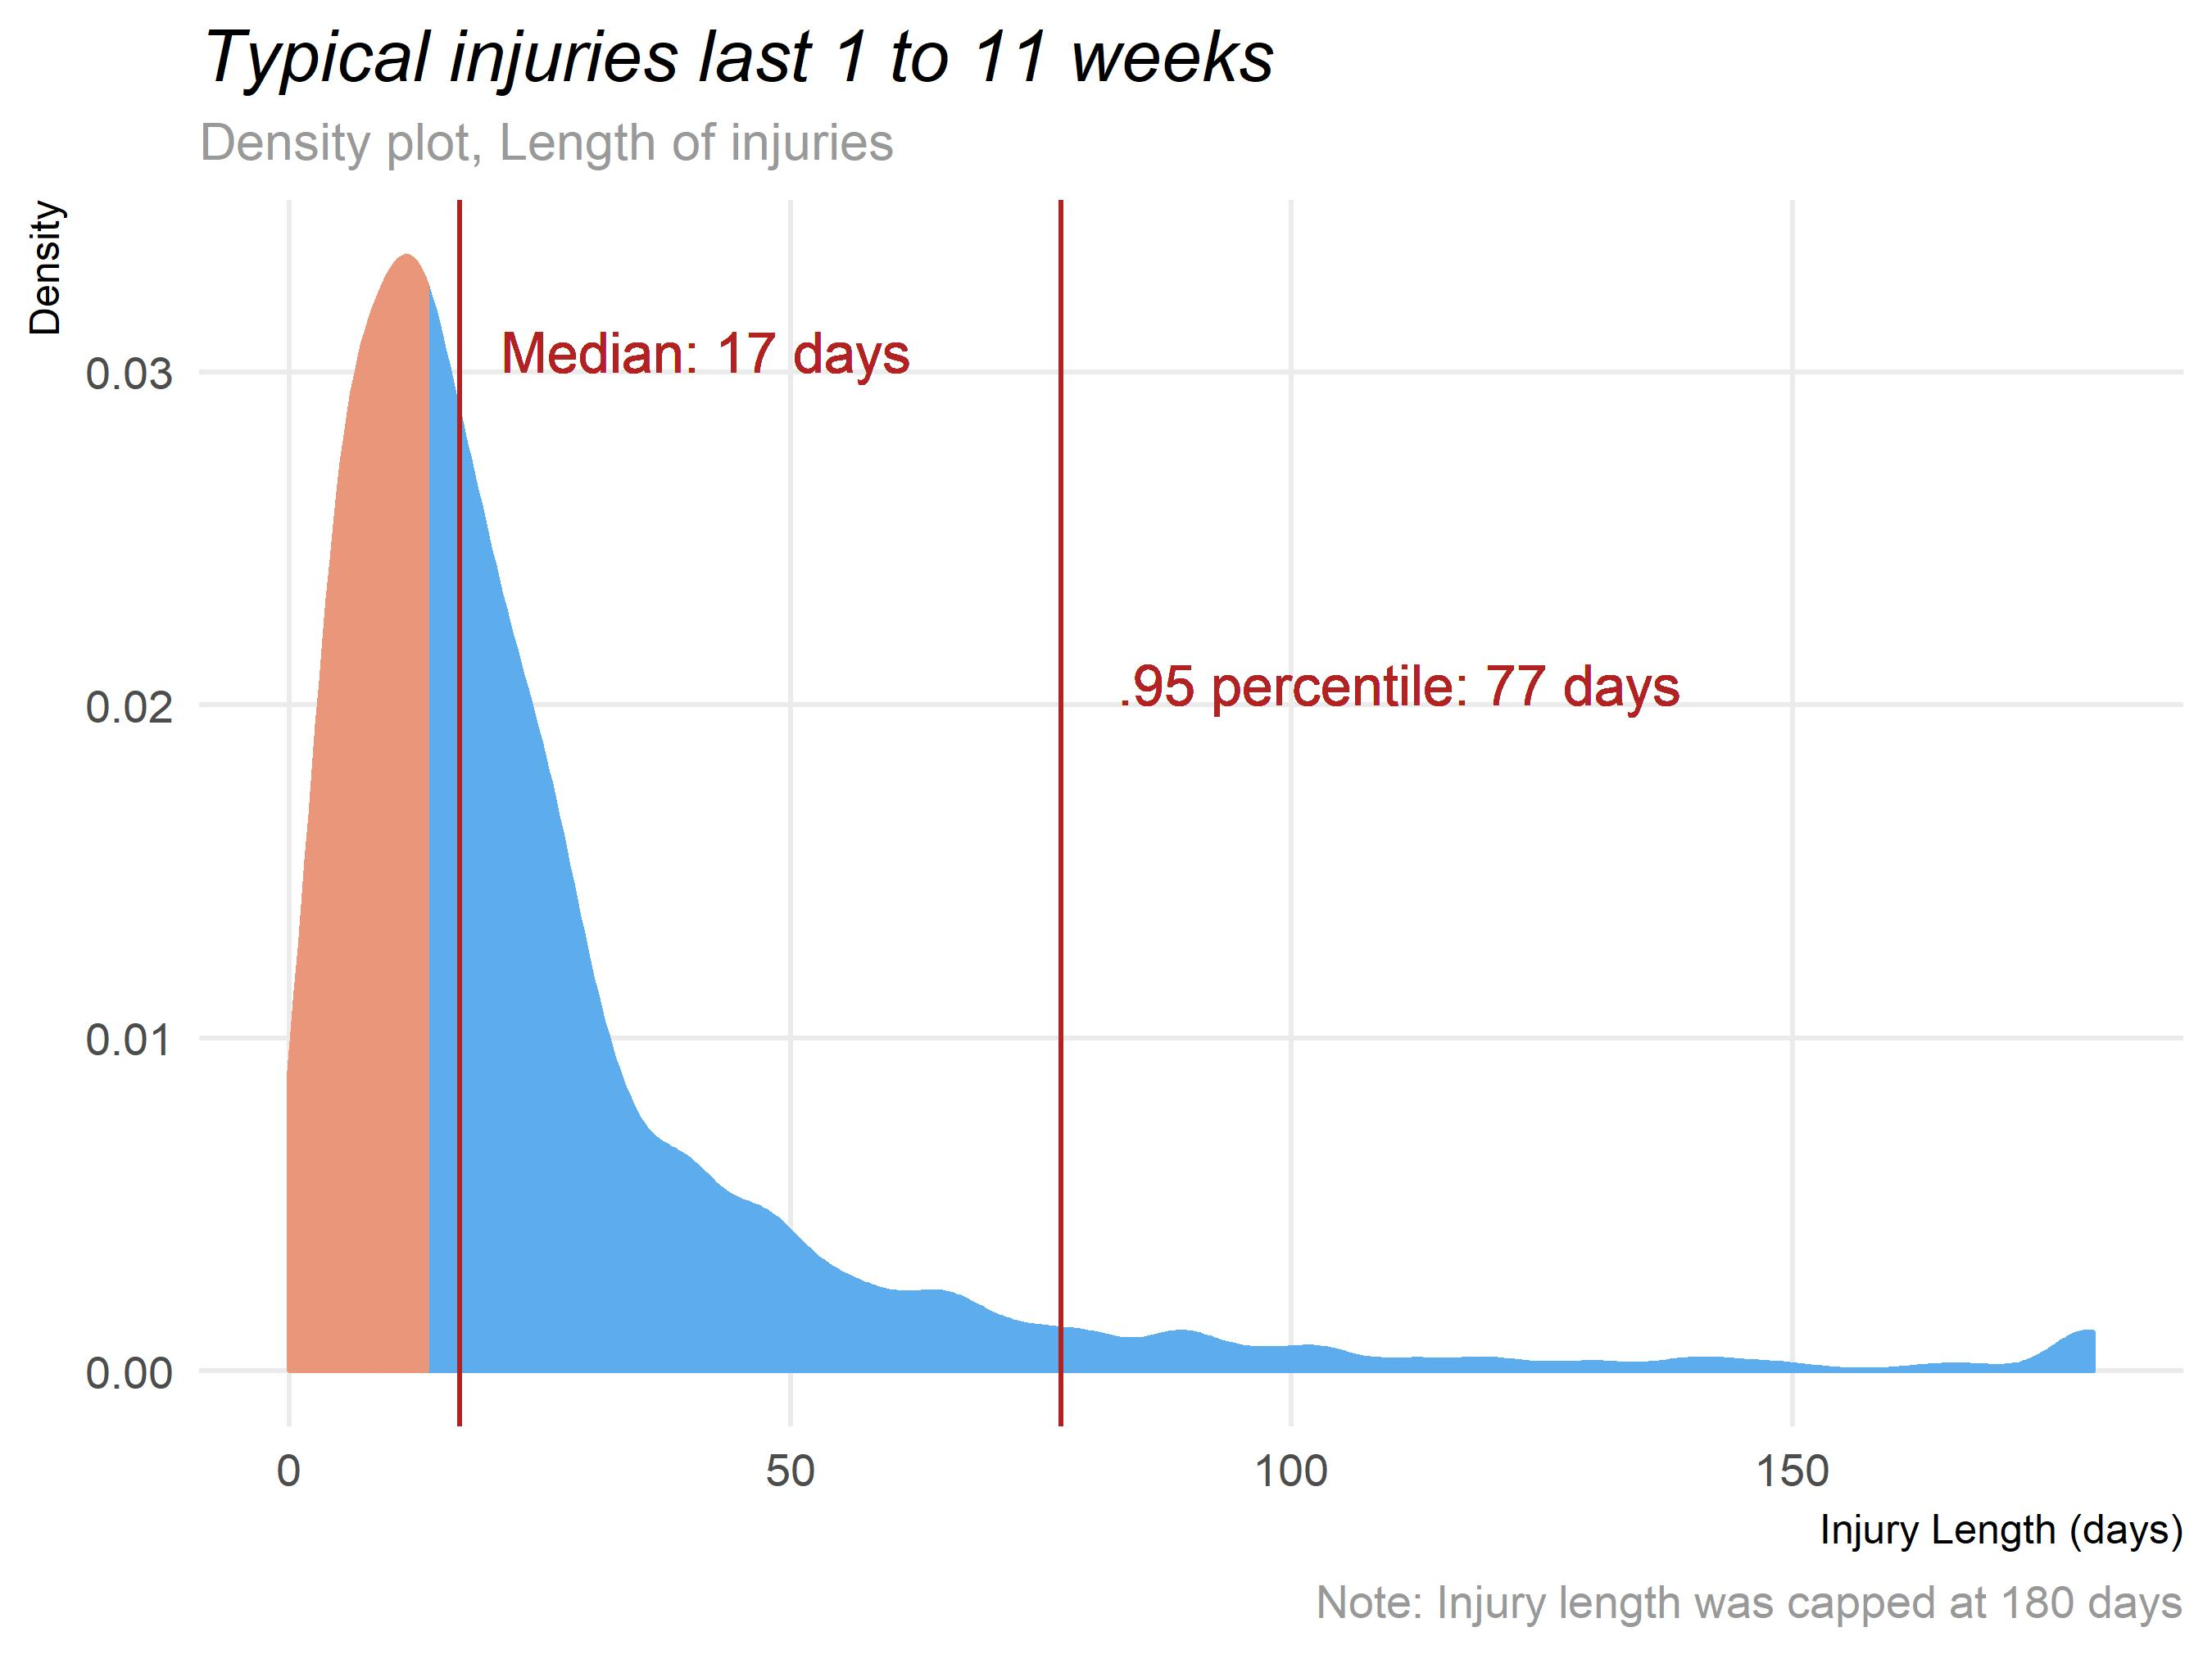
\includegraphics[width=0.5\linewidth]{C:/Users/tkonc/Documents/pl_injuries/Figures/4. Hamstring Injury Lengths} \end{center}

\paragraph{Position}\label{position}

{\#\#TODO: write about position filters}

\paragraph{Playing time}\label{playing-time}

\#\#TODO: explain why it wasn't applied/span\textgreater{}

\paragraph{Missing data}\label{missing-data}

{\#\#TODO: explain how it was handled in different cases}

\begin{itemize}
\tightlist
\item
  Foot
\item
  Position
\item
  Games played
\end{itemize}

\subsection{Feature Engineering}\label{feature-engineering}

There are certain variables that were not available in the raw data
format, however they could be calculated / extracted, with the aim of
enhancing the analytical separation between injured / non-injured cases.

Below is a comprehensive list of all variables created during the data
preparation:\\
* Weekday and Month\\
* BMI\\
* Team and Opponent\\
* Birthplace and Nationality\\
* Kick-off time\\
* Injured \ldots{}\\
* Games \ldots{}\\
* Groupings\\
* Polinomial terms

{\#\#TODO: explain logic for each}

\emph{An important technical note on categorical variables: before
feeding them into predictive models, all categoricals were
dummy-encoded.}

\subsection{Exploratory Analysis}\label{exploratory-analysis}

\subsection{Separation of data sets}\label{separation-of-data-sets}

\section{Modeling}\label{modeling}

\subsection{The problem of class
imbalance}\label{the-problem-of-class-imbalance}

\section{Appendix}\label{appendix}

\subsection{Project organization}\label{project-organization}

This project is breaken into separte, runable parts, which are not
included in this markdown file.\\
The main parts are:\\
1. Raw Data\\
2. Runable R scripts, storing the steps of the analysis\\
3. Functions\\
4. Models\\
5. Notebooks\\
6. Figures\\
7. Data

{\#\#TODO: add details}

\subsection{List of variables in raw
data}\label{list-of-variables-in-raw-data}

\begin{longtable}[]{@{}ll@{}}
\toprule
Variable & Description\tabularnewline
\midrule
\endhead
Date & date of the game (YYYY-MM-DD)\tabularnewline
balance & absolute full time goal difference=\textbar{}ft\_a -
ft\_h\textbar{}\tabularnewline
ft\_a & full time away team goals\tabularnewline
ft\_h & full time home team goals\tabularnewline
Attendance & number of fans at the game\tabularnewline
Game week & game week of the season\tabularnewline
Kick-off & kickoff time (GMT)\tabularnewline
Venue & Location of the stadium\tabularnewline
home & whether player lines up or the home side or not\tabularnewline
ht\_a & half time away team goals\tabularnewline
ht\_h & half time home team goals\tabularnewline
injured & whether player was reported injured after the match, (before
playing any other match) or not\tabularnewline
mid & unique match id\tabularnewline
minutes & minutes played by the player on the match (stoppage time is
discarded, so cannot be more than 90)\tabularnewline
pid & unique player id\tabularnewline
starter & whether player started the match or not\tabularnewline
injury\_length & if player was reported after the game, how many days
did the injury reportedly last\tabularnewline
injury\_type & what type of injury was reported\tabularnewline
injury\_minutes\_played & equals the minutes variable in case of injured
= 1, otherwise 0\tabularnewline
days\_till\_injury & how many days between the date of the match and
start of reported injury\tabularnewline
pl/all\_minutes/games\_n/season & how many games/minutes of premier
league/any other football played by player in the n/days before the
match (or in the season, total)\tabularnewline
Country of birth & player country of birth\tabularnewline
Date of birth & player DoB\tabularnewline
First name & player first name\tabularnewline
Foot & player preferred foot\tabularnewline
Height & player height\tabularnewline
Last name & player last name\tabularnewline
Nationality & player nationality\tabularnewline
Place of birth & player place of birth\tabularnewline
Position & player position\tabularnewline
Weight & player weight (at time of collecting data)\tabularnewline
away\_team & away team name\tabularnewline
away\_tid & away team id\tabularnewline
home\_team & home team name\tabularnewline
home\_tid & home team id\tabularnewline
\bottomrule
\end{longtable}

\subsection{Sessioninfo}\label{sessioninfo}

\begin{verbatim}
## R version 3.5.1 (2018-07-02)
## Platform: x86_64-w64-mingw32/x64 (64-bit)
## Running under: Windows 10 x64 (build 17134)
## 
## Matrix products: default
## 
## locale:
## [1] LC_COLLATE=English_United States.1252 
## [2] LC_CTYPE=English_United States.1252   
## [3] LC_MONETARY=English_United States.1252
## [4] LC_NUMERIC=C                          
## [5] LC_TIME=English_United States.1252    
## 
## attached base packages:
## [1] stats     graphics  grDevices utils     datasets  methods   base     
## 
## other attached packages:
## [1] knitr_1.20
## 
## loaded via a namespace (and not attached):
##  [1] compiler_3.5.1  backports_1.1.2 magrittr_1.5    rprojroot_1.3-2
##  [5] tools_3.5.1     htmltools_0.3.6 yaml_2.1.19     Rcpp_0.12.17   
##  [9] stringi_1.1.7   rmarkdown_1.10  highr_0.7       stringr_1.3.1  
## [13] digest_0.6.15   evaluate_0.11
\end{verbatim}


\end{document}
